\subsection{Planetary-shell fields}
\label{man:planetary-shell-fields}

This section records retained-shell forms for later planetary and ring-family examples. Phase~IV provides manual-local scaffold rows and tests for source hygiene. It does not promote the shell rows to validated predictions.

\subsubsection{Earth water--atmosphere--Moon shell witness}
\label{man:earth-water-atmosphere-moon-shell-witness}

\RetentionBlock
{Earth water-atmosphere-Moon retained shell field}
{water + atmosphere + Moon boundary shell}
{external sector and material benchmark layers}
{basin geometry + solar boundary + atmospheric circulation shell}
{shell scaffold window only}
{pending until script/test-backed shell rows are declared}

The retained parent field is
\[
\mathcal O_{\oplus\text{-Moon}}=
\mathcal O_{\mathrm{solid\ Earth}}
\cup
\mathcal O_{\mathrm{water}}
\cup
\mathcal O_{\mathrm{atmosphere}}
\cup
\mathcal O_{\mathrm{Moon}}
\cup
\mathcal O_{\mathrm{near\ space}}.
\]
The retained extraction is
\[
\mathcal F_K=
\mathcal O_{\mathrm{water}}
\cup
\mathcal O_{\mathrm{atmosphere}}
\cup
\partial\mathcal O_{\mathrm{Moon}}.
\]
The first refinement is
\[
\mathcal F_{K+1}=\mathcal F_K+
\text{basin geometry}+
\text{solar boundary}+
\text{atmospheric circulation shell}.
\]
A planetary-shell row has the form
\[
Q_{\oplus\text{-Moon}}^{(\ell,\omega)}=
(\Phi_{\mathrm{water}},\Phi_{\mathrm{atm}},\chi_{\oplus},
Q_{\mathrm{water}},S_{\mathrm{water}},
Q_{\mathrm{atm}},S_{\mathrm{atm}},
R,R_0,T,T_0,B^*,\widehat\Lambda,
P_{\mathrm{shell}},P_{0,\mathrm{shell}},\Sigma_{\mathrm{shell}}).
\]
The pair \((Q,S)\) in this scaffold records the boundary-polarization count pair of the retained shell extraction.

\begin{table}[H]
\centering
\caption{Phase IV Earth--Moon shell scaffold rows.}
\label{tab:earth-moon-shell-phaseiv-rows}
\begin{threeparttable}
\small
\begin{tabularx}{\linewidth}{@{}lcccccX@{}}
\toprule
Component & \(\Phi\) & \(\chi\) & \(Q/S\) & Loss & Torsion & Topology tag \\
\midrule
water shell & \(34/5\) & \(+1\) & \(2/17\) & \(11/12\) & \(6/5\) & planetary.water.boundary \\
atmosphere shell & \(21/4\) & \(-1\) & \(-1/19\) & \(13/15\) & \(9/7\) & planetary.atmosphere.boundary \\
Moon boundary & \(13/3\) & \(+1\) & \(1/23\) & \(17/18\) & \(9/8\) & planetary.moon.boundary \\
\bottomrule
\end{tabularx}
\ManualTableNote{The \(Q/S\) column is a boundary-polarization count-pair report for the retained shell row.}
\end{threeparttable}
\end{table}

\begin{figure}[H]
\centering
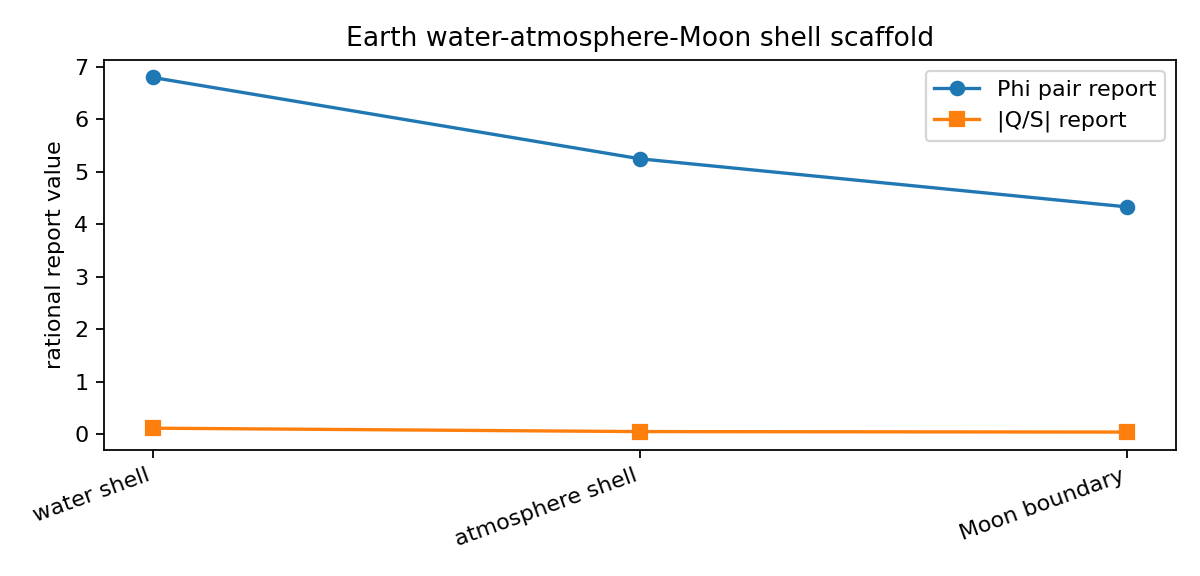
\includegraphics[width=0.82\linewidth]{figures/planetary/01_earth_moon_shell_scaffold.png}
\caption{Earth water-atmosphere-Moon retained-shell scaffold.}
\label{fig:earth-moon-shell-scaffold}
\end{figure}

\subsubsection{Saturn and galactic ring-refinement scaffold}
\label{man:saturn-galactic-ring-refinement-scaffold}

Phase~IV also records the shared ring-family refinement shape used by the Saturn shell row and the galactic outer-shell row. The refinement remains source-normalized or scaffolded until the corresponding application scripts and source maps are declared.

\begin{table}[H]
\centering
\caption{Ring-family refinement scaffold.}
\label{tab:ring-refinement-scaffold}
\begin{threeparttable}
\small
\begin{tabularx}{\linewidth}{@{}lXcccX@{}}
\toprule
Family & Retained extraction & Witness & Phase lock & \(B^*\) & Status \\
\midrule
Saturn ring-moon shell & D--E ring family + selected moons & Cassini Division & \(3/7\) & 144 & scaffold \\
Galactic outer-shell family & outer-orbital shell witness set & outer-shell band & \(5/9\) & 137 & source-normalized pending \\
\bottomrule
\end{tabularx}
\ManualTableNote{The phase-lock entries are rational row reports; benchmark comparison requires a named source-normalization map.}
\end{threeparttable}
\end{table}

\begin{figure}[H]
\centering
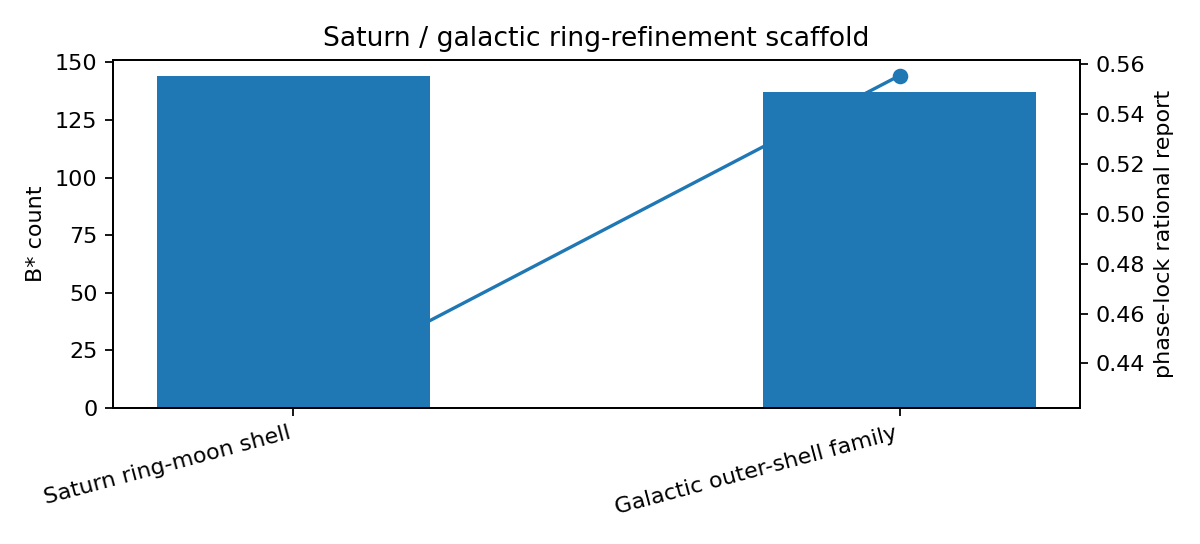
\includegraphics[width=0.82\linewidth]{figures/planetary/02_saturn_galactic_ring_refinements.png}
\caption{Saturn and galactic ring-refinement scaffold rows.}
\label{fig:saturn-galactic-ring-refinement}
\end{figure}

\paragraph{Reproducibility.}
The raw setup, script, derived CSVs, figures, and tests are manual-local. They are listed in the manual artifact map and audited by the Phase IV application-scaffold audit.
